\chapter{State of the art}
\label{sec:chapter2}
\thispagestyle{empty}

 This chapter reports an overview of research works regarding the task of door finding performed by autonomous robots. We start by discussing the usefulness of door detection for robotics applications, reporting some challenging tasks for autonomous agents, and how they can benefit from door detection. Then, we report the most relevant door detection approaches based on handcrafted features extracted from visual data. Due to the predominant role that Deep Learning methods have acquired in Computer Vision tasks (like image classification and segmentation, scene understanding, and object detection), we survey the evolution of end-to-end methods to perform object detection, reporting also some preliminary concepts of Machine and Deep Learning that are of interest for this work. Then, we present relevant approaches to detect doors by mobile robots that exploit the advantages of deep models. The next section of this chapter surveys the open problems and challenges of Deep Learning applied to robotic vision applications. Finally, we define the importance of simulations to acquire well-formed datasets for training and testing end-to-end models engaged in robotics contexts.  
 
 \section{The Utility of Door Detection for Mobile Robots}
 
 Doors are useful semantic features for an active agent. By collecting information about doors, a robot can improve significantly its knowledge about the environment in which it operates. Exploration and navigation, two of the main tasks performed by a mobile robot, can be strongly influenced by exploiting knowledge about doors, such as their location and status (e.g. closed or opened). 
 
 Exploration is the task in which an autonomous agent incrementally discovers features of interest in an initially unknown environment. Typically, an autonomous agent builds a map of the environment to perform navigation.  Map acquisition enables autonomous agents to navigate inside a previously unknown environment. With this procedure, a robot builds a metric map of the indoor environment it is exploring. A metric map is represented by an occupancy grid: a two-dimensional matrix in which each cell represents a sub-portion of the environment and contains the probability that the portion is occupied by an obstacle or it is free. Occupancy grids were first proposed in \cite{cuupancygridfirst} and they have become widely used for mobile robot localization, exploration, and navigation \cite{gridmapnavigation, ariel, girdmapexploration}. A way to store and visualize occupancy grid maps is to encode them in an 8-bit gray-scale image, normalizing the probability values of the cells to the range between 0
 and 255. A further simplification in the binary occupancy grids (Fig. \ref{fig:binary_grid_map}), where each cell has a boolean value representing the occupancy status. An occupied location is represented as \textit{True} (1) while free spaces are tagged with \textit{False} (0). Collecting data about doors can improve the mapping strategy followed by mobile robots. By detecting closed doors locations by mapping, an agent can guess what floor areas are temporarily unreachable, and can consequentially act to collect the entire environment map. For example, it can open the door through a robotic arm \cite{doorcabinet} or ask help to a human operator. Another solution concerns identifying the presence of unreachable locations by detecting closed door and making a map refinement in future stages (when closed doors are eventually opened).
 
 Room segmentation divides grid maps into semantically meaningful regions making the pure spatial environment model, provided by grid maps, more informative. Fig. \ref{fig:room_segmentation_map} shows an occupancy grid map divided into rooms. \citeauthor{segmentationsurvey}, \cite{segmentationsurvey}, survey the literature regarding room segmentation and provide a comparison of the most relevant methods. In \cite{segmenationfornavigation}, the authors argue that room segmentation yields significant savings in computational efforts for obtaining navigation trajectories . Likewise, the work presented \cite{segmentationhumanrobot} demonstrates that human-robot communication greatly benefits from a high-level room's division. Furthermore, cleaning agents can exploit room maps to improve their navigation strategy by creating an efficient cleaning path throughout the floor plan, as explained in \cite{segmentationcleaning}. While spatial mapping has been extensively investigated and several automatized tools have been proposed, the research community is still investigating robust methods for obtaining accurate room-level segmentation of an indoor environment. The sensors' perception is inaccurate; noise and missing data introduce several errors in robot perception. Furthermore, indoor environments are highly cluttered with furniture and other objects. Separating clutter from permanent structures such as walls and doors is difficult as furniture can occlude crucial structural features. Robust door detection can improve the grid maps segmentation providing useful information of connections between different rooms.
 
 \begin{figure}[h!]
 	\centering
 	\begin{subfigure}[b]{0.45\linewidth}
 		\centering
 		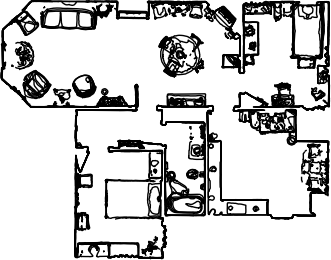
\includegraphics[width=\textwidth]{images/occupancygrid.png}
 		\caption{Binary occupancy grid map.}
 		\label{fig:binary_grid_map}
 	\end{subfigure}
 	\hfill
 	\begin{subfigure}[b]{0.48\linewidth}
 		\centering
 		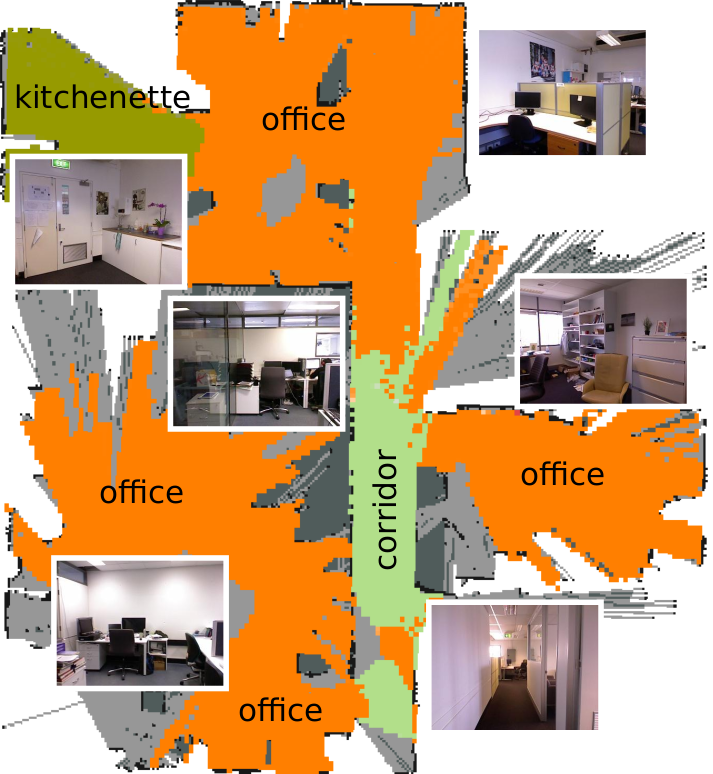
\includegraphics[width=\textwidth]{images/semanticmap.png}
 		\caption{Semantic map \cite{placecategorization}.}
 		\label{fig:semantic_map}
 	\end{subfigure}
 	\newline
 	\newline
 	\begin{subfigure}[b]{0.99\linewidth}
 		\centering
 		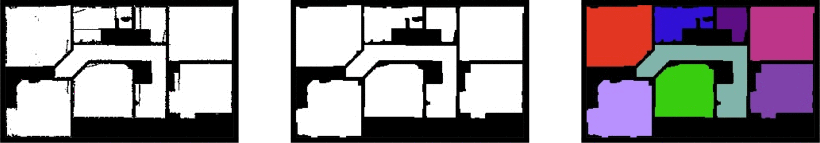
\includegraphics[width=\textwidth]{images/roomsegmentation.png}
 		\caption{Room segmentation map \cite{segmentation3d}.}
 		\label{fig:room_segmentation_map}
 	\end{subfigure}
 	\caption{Three different types of maps.}
 	
 \end{figure}
 
 The room level map obtained through room segmentation can be further improved by exploiting scene recognition or place categorization. This task consists of semantically labeling indoor scenes, such as an ``office'', a ``kitchen'', or a ``bedroom''. Through place categorization, an autonomous agent builds a semantic map (an example is shown by Fig. \ref{fig:semantic_map}), in which any environment location is tagged with a label. In literature, there are a lot of studies concerning place categorization by autonomous agents \cite{scenerecognitionaudio, scenerecognitiononjectdetection, placecategorization, placecategorizationlargescale}. These approaches collect useful information from the scenes (like audio signals or RGB images), then classify these data to divide the environment into rooms, and finally assign a semantic label to each place. One of the main problems is to correctly segment the environment into rooms. This is because data acquired in different rooms can be similar (in this case adjacent rooms can be considered as the same semantic place) or the same room can present different features which can result in an incorrect division of a single room. Identifying the rooms' connections and estimating their location allows mobile robots
 to robustly identify different rooms. Furthermore, door detection can help these methods to find the precise location in which a semantic place ends and another room begins, performing a more refined place segmentation and categorization.  
 
 Another task that can get benefit from door detection is Semantic SLAM (Simultaneous Localization and Mapping). Semantic SLAM aims to build a semantic map online during exploration without a complete and previously-acquired knowledge of the environment. Recent Semantic SLAM methods combine classical geometry-based estimation with Deep Learning-based object detection. The work presented in \cite{semanticslamsurvey} surveys and evaluates the most relevant approaches that perform Semantic SLAM. The authors argue that semantic segmentation is the largest source of error in the analyzed methods. Doors are useful semantic features of indoor environments and their detection can be added in Semantic SLAM approaches. Furthermore, door detection can improve the segmentation accuracy performed in previous stages, because the robot can robustly group the data acquired in different rooms. 
 
 Another task that can be improved by exploiting doors recognition is navigation. The authors of \cite{sonarandivisualdoordetection} propose a method to anticipate the door's crossing during navigation, in order to improve the door traversing task. A similar approach is presented in \cite{doorsandnavigation}, where \citeauthor{doorsandnavigation} describe a method for finding doors online during navigation, facilitating how a robot approaches doors. These works prove the usefulness of doors' data for navigation in autonomous agents.
 
 \section{Doors Detection using Handcrafted Features}
  In literature, there are a lot of different studies concerning door detection. One of the firsts attempts, described in \cite{sonarandivisualdoordetection}, combines visual information and sonar sensors to safely traverse doors by a B21 robot. Doors present a challenging obstacle for this agent, so the goal consists of traversing opened doors using a certain angle to avoid collisions. This activity is divided into two sub-tasks: door detection and door crossing. The first one is of interest to this thesis. \citeauthor{sonarandivisualdoordetection}, \cite{sonarandivisualdoordetection}, consider an opened door as a squared noisy rectangular segment in an image. To detect it, this approach applies a vertical Sobel Filter to the grayscaled image. If it is detected a column wider than a certain threshold, it is considered a door. The sonar sensors are used to obtain the robot's distance from possible doors, to confirm the matches and avoid false positives (wrong recognition of doors).
  
  The method of \cite{humanoid} proposes a solution to detect both a door and its knob by a humanoid robot. This solution recognizes the door's features and works sufficiently fast to perform online. \citeauthor{humanoid} \cite{humanoid} argue that a door does not have very discriminative features, and the door's appearance can vary dramatically as viewpoint changes. To solve this issue, the proposed method at first extracts features points from input frames using an optimized version of the CenSurE filter, described in \cite{censure}. Then, the Randomized Tree algorithm classifies these features to determine if a frame contains a door (the approach is reported in \cite{treefeature}). The tree predictor is trained offline using the feature points extracted from \emph{base images} previously acquired in the real environment. If a door is detected, the robot walks toward the door and localizes its knob using a segmentation technique and some general constraints (size, ratio, and height bounds).
  
\begin{figure}[h!]
	\centering
	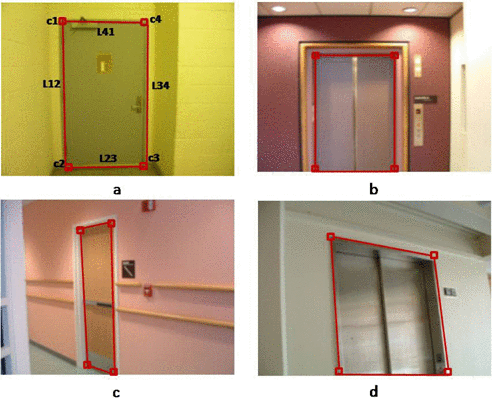
\includegraphics[width=0.75\linewidth]{images/corner_door.png}
	\caption{The geometric model of a door (a). The ideal model (b).   The model with occlusion (c) and perspective deformation (d). Image from \cite{cornerdetector}.}
\end{figure}
  
  Another method for recognizing doors in unfamiliar environments is described in \cite{edgeandcornerdoorsdetector}. In this work, doors are considered significant landmarks for navigation and self-localization not only for an autonomous agent but also for blind people. This method takes into account of a variety of conditions, including differences in illumination, scale changes, deformation caused by perspective and occlusion, and variance of doors’ color, texture, or appearance.  
   At first, images are converted in grayscale and smoothed by Gaussian lowpass filter. Then, edges and corners are extracted from the pre-processed frames, using respectively the Canny Edge Detector, \cite{canny}, and the method described in \cite{cornerdetector}. The authors then define a geometric shape model of doors, which is composed of two horizontal and two vertical lines between four corners. These features are then aggregated to find possible doors: only those groups that match the model are considered as true positives.  
   
\section{Machine Learning Preliminaries}
\label{sec:machine_learning}

This thesis approaches the problem of detecting doors as well-known Computer Vision task: object detection. Today, Computer Vision strongly depends on the power of Deep Learning \cite{deeplearningoverview}.
Deep Learning is a sub-field of Machine Learning, which is the study of computer algorithms that can improve automatically through experience by the use of data.  It is a powerful technique suitable when it is not feasible to develop a standard algorithm to solve a difficult task. For example, in the context of this thesis, we use Machine Learning to detect doors in RGB images. A \textit{learning algorithm} uses sample pairs of training data to create a model, also called predictor, that is able to classify other unseen data. The first important aspect for a machine learning problem is the dataset. Typically, a dataset is composed of pairs of data taken from two different domains: the \textit{data space} and the \textit{label set}.

\begin{definition}[Data domain]
	The data domain, denoted as $\mathcal{X}$, is the set of all possible data points for a given learning problem. Each data point is defined by features. In some cases, the features are encoded as vectors of real numbers. Such a representation is called \textit{natural} because the data consist of homogeneous quantities, like pixels in an image or words' frequencies in a document. A data point is denoted as $x \in \mathcal{X}$ and it is defined as a vector of features $x = (x_1, ..., x_d)$.
\end{definition}

\begin{definition}[Label set]
	$\mathcal{Y}$ denotes the set of all possible labels that a data point can assume. For a classification problem, the label set is typically finite and small (such as $\mathcal{Y} = \{\text{sport}, \text{politics}, \text{business}\}$ for a categorization task on documents). Otherwise, for a regression task, the label set is typically equal to $\mathbb{Q}$, which is the rational numbers' set. In this case, the label set is infinite.
\end{definition}

In a \textit{supervised} learning problem, the data points are tagged with their respective ground-truth labels. In particular, the dataset's entries are pairs $p = (x, y)$, where $x \in \mathcal{X}$ is a data point and $y \in \mathcal{Y}$ is the label assigned to it. A \textit{supervised} learning algorithm is a technique that aims to build a model learned from a \textit{training set}. This paradigm is called \textit{learning by examples}. An example is a pair $p=(x, y)$, where $x$ is a data point represented by a vector of features and $y$ is its ground-truth label, while the training set is composed of a series of examples $S=\{(x_1, y_1), ..., (x_m, y_m)\}$. A \textit{supervised learning algorithm} for \textit{learning by examples} receives a training set and outputs a learned model.

\begin{definition}[Model]
	A model is a function $f:\mathcal{X} \to \mathcal{Y}$ that maps data points to labels. 
\end{definition}

The training examples come from some generally unknown probability distribution and the goal of a learning algorithm is to infer a function that approximates this distribution (or makes a generalization of it) to produce sufficiently accurate predictions in new cases. During the training procedure, the examples (that are pair $p = (x, y)$ where $x$ is the data point and $y$ is its ``true'' label) are fed into the model to be classified. At each step, the goodness of the model's predictions is measured through the loss function. Then, according to the loss function's value, the internal representation of the model is adjusted to produce more refined predictions.

\begin{definition}[Loss function]
	A loss function $\ell(y, \hat y)$ measures the discrepancy between the predicted label $\hat y$ and the ground-truth label $y$. In a correct prediction the loss function's values is $0$: $\ell (y, \hat y) = 0$.
\end{definition}

Informally speaking, a model represents a function $f$ that generate predictions $\hat y = f(x)$ minimizing the loss function $\ell(y, \hat y)$ over the data points $x \in \mathcal{X}$. In practice, the function $f$ is determined by a certain configuration of parameters and/or the internal structure of a learning model.

In order to estimate the predictive power of a model, we typically use a \textit{test set}. This is a set of examples $T=\{(x_1', y_1'), ..., (x_n', y_n')\}$ to which the learning algorithm does not have access during the training phase. During the test procedure, each pair in the \textit{test set} is fed into the model in order to measure the goodness of each prediction compared with the ground-truth label. This quantity is measured by the \textit{loss function}. 

The test set allows to determine the predictive power of a learned model on unseen new data. To measure the goodness of a predictor, we can calculate the \textit{test error} over a test set $T$. Given a loss function $\ell$, the test error is
\begin{equation}
\frac{1}{n} \sum_{s=1}^{n}\ell(y_s', f(x_s'))
\end{equation}
where $n$ is the test set's cardinality ($n = |S|$), $y_s'$ is the ground-truth label of the s-th test example and $f(x_s')$ returns the label of the s-th data point produced by the predictor $f$. Since the test set is disjoint from the training set and emulates the unseen data, it cannot be used during the learning phase.

A way to train a learning model is the Empirical Risk Minimization (ERM) approach. ERM offers a theory to design learning algorithms that generate predictors with a low test error considering only the training set. ERM assumes that the \textit{training error} (the error computed over a training set $T$) of a predictor is directly correlated to its test error. The training error is given by:

\begin{equation}
\hat \ell(f) = \frac{1}{m} \sum_{t=1}^{m}\ell\big{(}y_t, f(x_t)\big{)}
\end{equation}
where the $m$ is the training set's cardinality ($m = |T|$).

\begin{definition}[Empirical risk minimization] 
	Let $\mathcal{F}$ a set of predictors and $\ell$ a loss function. The empirical risk minimizer (ERM) is the learning algorithm that outputs some predictor $f \in \mathcal{F}$ minimizing the training error:
	
	\begin{equation}
	\hat f \in \argmin_{f \in \mathcal{F}} \hat \ell(f),
	\end{equation}
	where $\in$ denotes there could be multiple $f \in \mathcal{F}$ that minimize the training error.
\end{definition}

The ERM algorithm fails when no predictors in $\mathcal{F}$ have a low test error, in particular when

\begin{equation}
\min_{f \in \mathcal{F}} \frac{1}{n} \sum_{s = 1}^{n} \ell(y_s', f(x_s'))
\end{equation} 
is high. The two main ways of failing for a generic learning algorithm are:
\begin{itemize}
	\item \textbf{underfitting:} when a learning algorithm tends to outputs predictors whose both test and training errors are high and close to each other. This means that possible predictors are unable to correctly classify the samples in the training set as well as those in the test set. This situation could depend on the training test size: if it is too small it can not represent well the data points' distribution or $\mathcal{F}$ (the set of the possible predictors) are too large with respect to the training set dimensions. Another reason that causes underfitting is the cardinality of $\mathcal{F}$. If the set of the possible predictors is small, there could not be a subset of them with a small test error. This means that the learning algorithm is not complex enough to output good learned models. In other words, when a model underfits it is not able to represent well the problem, failing to classify examples from both training and test sets;
	\item \textbf{overfitting:} when a learning algorithm tends to output predictors whose training error is low (or it tends to zero) while the test error is high. In this situation, the predictors produced by a learning algorithm learn too much from the training data and, as a result, are unable to produce good predictions on new data. This means that those predictors do not generalize the problem, but are specialized in dealing only with the data used during the training phase.
\end{itemize}

When $A$ is an ERM learning algorithm and the size $m$ of the training set is fixed, we should expect overfitting when $\log_2|\mathcal{F}| \gg m$, so the set of possible predictors is too large with respect to the training set's size. On the other hand, when $\log_2|\mathcal{F}| \ll m$ we should expect underfitting.

\section{Deep Learning Preliminaries}
Deep Learning is a sub-field of Machine Learning based on \textit{neural networks}. This learning algorithm is inspired by the information processing and the distributed communication of biological brains. Neural networks (NNs) are a large and complex class of predictors, based on artificial neurons.

\begin{definition}[Neuron]
	An artificial neuron is a mathematical function inspired by biological neurons, which represents the elementary units in an artificial NN. The mathematical function implemented by a neuron is $g(x) = \sigma(\omega^\intercal \cdot x)$, where $\sigma$ is the (non-linear) activation function, $\omega$ is the weight vector of the learnable parameters, and $x$ is the input vector of the neuron. This means that each input is separately weighted and the sum is passed through a non-linear function. The activation function usually has a sigmoid shape and often it is monotonically increasing, continuous, and bounded. A single neuron can approximate only linear functions.	
\end{definition}

Artificial neural networks are composed of a series of simple predictions made by neurons. The adjective ``deep'' in Deep Learning refers to the use of multiple layers in NNs. The most simple model of neural networks is called feed-forward. 

\begin{definition}[Feed-forward neural network]
	A feed-forward neural network computes functions of the from $f : \R^d \to \R^n$. Its structure is a directed acyclic graph $G = (V, E)$, in which $V$ is the set of nodes (neurons) and $E$ is the set of edges that connects the neurons. The presence of multiple neurons allows the neural network to infer non-linear functions. The vertices in $V$ are divided into three subgroups: $V = V_{in} \cup V_{hid} \cup V_{out}$, where $V_{in}$ (with $|V_{in}| = d$:	 the feature space's dimension) are the input nodes which have no incoming edges, $V_{out}$ (with $|V_{out}| = n$, the number of labels) are the output nodes which have no outgoing edge, and $V_{hid}$ are the hidden nodes, which have both incoming and outgoing edges.
\end{definition}

The most simple form of the feed-forward neural network is the multi-layer perceptron (MLP), in which the nodes of $V$ is partitioned in a sequence of consecutive layers such that each node of a layer has incoming edges only from
nodes in the previous layer and outgoing edges only to nodes of the next layer.  The layers containing the hidden nodes are called hidden layers. The learnable parameters are the weights assigned to the edges between neurons. 
A parameter $\omega_{i,j} \in \R$ (called weight) is associated with every edge pair $(i, j) \in E$.  We use $W$ to denote the $|V | \times |V |$ weight matrix, where $(i, j) \notin E$ implies $\omega_{i,j} = 0$. The graph $G$, the weights matrix
$W$, and the activation function $\sigma$ define the function $f = f_{G,W,\sigma}$ computed by the network.  Note that when $n = 1$ (one output node) and $|V_{hid}| = 0$ (no hidden nodes), then $\mathcal{F}_{G,\sign}$ only contains linear classifiers of the form $f(x) = \sign(\omega^\intercal \cdot x)$. 

The training of neural networks is not trivial. The most natural approach for training a model in $\mathcal{F}_{G,\sigma}$ is ERM, as mentioned in Sec. \ref{sec:machine_learning}.
Unfortunately, this method could not be efficiently applied to neural networks. The following theorem confirms this statement.

\begin{theorem}
	For every integer $k \geq 3$, let $G$ be a network with $d$ input nodes, a single hidden layer containing $k + 1$ nodes (one of which has a constant value 1), and a single output node. Then the problem of minimizing the zero-one loss training error in $\mathcal{F}_{G,\sign}$ is NP-hard. 
\end{theorem}

The models considered by this theorem are simplified neural networks that solve \textit{binary classification} tasks using the zero-one loss (equation \ref{formula:zero-oneloss}) with a single hidden layer composed of four or more neurons. 

\begin{equation}
\label{formula:zero-oneloss}
\ell(y, \hat y) = 
\begin{cases}
0 & \text{if $y = \hat y$} \\
1 & \text{if $y \neq \hat y$}
\end{cases}
\end{equation}

This theorem demonstrates the inefficiency of ERM for a simple NN. This means that this theorem is true even for more complex neural networks and different tasks. ERM remains NP-hard even when $\mathcal{F}_{G,\sign}$ contains only linear classifiers (i.e. $G$ has no hidden nodes). However, while the cause of NP-hardness in linear models was the non-convexity of the loss function (zero-one loss in this case), in multi-layered neural networks the problem is inherent to their structure. The key observation is that the presence of hidden nodes in NN makes the loss function $\ell_t$ over an example $(x_t, t_t)$ non-convex in the weights matrix $W$ even when $\ell(x, y)$ is convex for all $y$. In general, the problem of minimizing a non-convex function is computationally intractable.  

This is because NNs are successfully trained even using algorithms that reduce the training error without any mathematical guarantee on the solution's quality. The training procedure starts with a forward propagation of the training examples in the neural network. After that, the outputs are used to quantify how good the predictions are and the error are back-propagated in the network using a descent algorithm. The standard algorithm for optimizing NNs is stochastic gradient descent (SGD):

\begin{equation}
\omega_{i, j} \leftarrow \omega_{i, j} - \eta_t \frac{\partial\ell_{Z_t}(W)}{\partial\omega_{i, j}} \quad \quad (i, j) \in E,
\end{equation}
where $Z_t$ is the index of a random training example and $\eta$ is an hyper-parameter that controls the step size (also called learning rate). The main idea is to calculate the partial derivative of the loss function, calculated on a training data point $t$ and the current NN status (described by the weights matrix $W$), over all the learnable parameters to adjust their values. In order to speed up convergence, the training samples can be grouped in mini-batches. Because the training error is a non-convex function of $W$, the SGD algorithm essentially finds only a local minima of the training error. The procedure to perform gradient descent on feed-forward NNs is known as \textit{error back-propagation}.
 
 \section{Deep Learning in Object Detection}
 As the performance of hand-crafted features based detectors are unable to increase \cite{deeplearningoverview}, Computer Vision researchers started to use Deep Learning methods for object detection. Today object detection strongly depends on the power of Deep Learning. \citeauthor{computervisionsurvey} in \cite{computervisionsurvey} survey the history of the most relevant approaches to perform this challenging task. 
 
 After the reborn of Convolutional Neural Networks (CNNs) in 2012, \citeauthor{rcnn} propose in \cite{rcnn} the first Deep Learning paradigm to detect objects, called RCNN (Region with CNN features). A RCNN, described in \cite{rcnn}, consists of three modules. The first generates category-independent region proposals, that are sub-portion of the same image. The second module is a large convolutional neural network (CNN) that extracts a fixed-length feature
 vector from each region. The third module is a set of class-specific linear SVMs, that predict the presence of an object within each region proposal using the relative feature vectors. Despite the great progress brought by RCNN, its drawback is obvious: the detection speed is extremely slow (about 14s per
 image with GPU). This is caused by the redundant feature computation over a large number of overlapped region proposals (over 2000 per image).
 
 To overcome this limitation, \citeauthor{sppnet} propose in \cite{sppnet} the Spatial Pyramid Pooling Networks (SPPNets). This new network computes a single feature map of the entire image and then associates these features to the correspondent region proposal. This method avoids the repeatedly feature extraction phase from overlapped sub-portions of the same image.  Unlike the classic CNNs, SPPNet accepts as input images of arbitrary size and generates a fixed-length representation regardless of image size/scale. 
 
 In \cite{fastrcnn}, \citeauthor{fastrcnn} describes a new detector called Fast RCNN. This work unifies in the single end-to-end module the CNN responsible to extract features and the bounding box regressor, improving training and testing speed while also increasing accuracy. 
 
 The next step is to generate object proposals directly with a CNN model. This technique is explained in \cite{fasterrcnn}, where \citeauthor{fasterrcnn} introduce Faster RCNN: the first near-realtime
 end-to-end Deep detector. The main contribution of this work is the Region Proposal Network (RPN) that simultaneously predicts object bounds and objectness scores at each position. Since that RPN is a convolutional network, it can be trained jointly with the entire model by sharing convolutional layers in a unique end-to-end learning framework. The training procedure alternates between fine-tuning for the region proposal task and object detection phase keeping the proposal regions fixed. 
 
 The methods described before are also defined ``two-stage detectors'', because they frame the detection as a ``coarse-to-fine'' process. Its evolution is a new paradigm called ``one-stage detectors'', where the detection process is performed in a single step.  In \cite{yolo}, \citeauthor{yolo} present YOLO (You Only Look Once), a novel neural network that doesn't follow the first detection paradigm based on ``proposal detection + verification''. YOLO, who is applied to the full image, divides a frame into a grid and predicts bounding boxes and class probabilities for each cell simultaneously. YOLO is also the first real-time detector: its runs at 45fps while a lighter implementation reaches 155 fps (though with less detection quality).  Later, several improvements have been made to YOLO. \citeauthor{yolov2}  proposed the v2 and v3 editions \cite{yolov2, yolov3}, improving both detection speed and accuracy.
 
  \begin{figure}[h!]
 	\centering
 	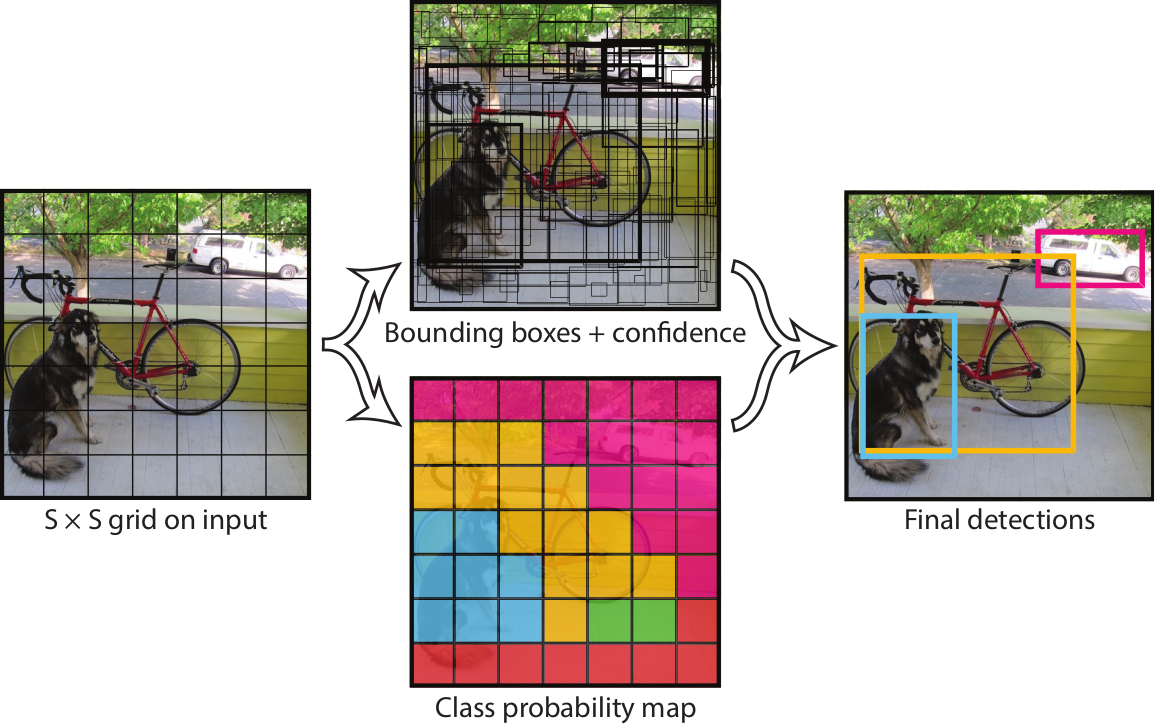
\includegraphics[width=\linewidth]{images/yolo.png}
 	\caption{The detection mechanism of YOLO, the first one-stage detector. YOLO models detection as a regression problem. It divides the image into an $S \times S$ grid and for each grid cell predicts $B$ bounding boxes, confidence for those boxes,
 	and $C$ class probabilities. These predictions are encoded as an
 	$S \times S \times (B * 5 + C)$ tensor. Image from \cite{yolo}.}
 \end{figure}
 
 Despite these great results, YOLO suffers from localization accuracy compared with two-stage detectors, especially for small objects. The second one-stage detector is called SSD (Single Shot MultiBox Detector), presented in \cite{ssd}. In this work, the authors introduce the multi-reference and multi-resolution detection techniques. The main idea is to define a set of anchor boxes with different scales and aspect ratios at different locations of the same image, and then predict the bounding boxes and their class using these references. Using this method, SSD significantly improves the detection performance, also for small objects. 
 
 Despite their fast computation, one-stage detectors are not yet able to overcome two-stage detectors in accuracy. In \cite{focalloss}, \citeauthor{focalloss} discover the reason behind this fact: it consists of the extreme foreground-background class imbalance encountered during training. Following this intuition, the authors propose in \cite{focalloss} a new loss function, called Focal Loss, to put more focus on hard misclassified examples during training. Thanks to Focal Loss, the one-stage detectors achieve an accuracy comparable to that of the two-stage detectors, while maintaining very high detection speed. In their work presented in \cite{focalloss}, \citeauthor{focalloss} design a simple end-to-end module called RetinaNet to demonstrate the effectiveness of their proposed loss function. 
 
 More recently in \cite{transformer}, \citeauthor{transformer} propose a new end-to-end paradigm called Transformer, who demonstrate state-of-the-art results in Natural Language Process tasks, e.g. text classification, machine translation, and question answering. Transformers are based on encoder-decoder architectures with self-attention mechanism. In a sequence of items, the self-attention technique estimates the relevance of each item to the others, capturing the interactions between them. This enables Transformers to model long dependencies between input sequence elements and support parallel processing. 
 
 This new architecture intrigued researchers to study its application to Computer Vision problems. In \cite{surveytransformer}, \citeauthor{surveytransformer} survey the history of Transformers' implication in Computer Vision. \citeauthor{detr}, \cite{detr}, present DETR (DEtection TRansformer), the first end-to-end model based on Transformer to perform object detection. DETR extracts features from an image using a CNN backbone and then feeds them into a classic transformer to capture their relationships. Its outputs are post-processed by a linear regressor and a multilayer perceptron, that infer the category labels and the bounding boxes, respectively.
 
 \section{Door Detection with Deep Learning} 
 Deep learning methods outperform traditional approaches in Computer Vision \cite{deeplearningoverview}. This is because classic methods based on handcrafted features are not generalizable, meaning the features (like edges or corners) needs to be specifically aggregated for different object categories. An end-to-end module, instead, learns automatically how to extract useful features that characterize an object. In particular, it extracts low-level features, corners or edges, in early stages, and then aggregates them in a more complex manner. It is well known that these features are robust to scale, shift, rotation, and exposure changes. Given their advantages, end-to-end modules have become widely used in robotics, including the task of door detection.
 
 The method proposed in \cite{detectdoorsfeature} is a vision-based technique for detecting doors by an autonomous agent. The main idea is to consider only color and shape information as useful features to detect doors in an office. This approach uses two neural classifiers to recognize these specific components in an image. One is trained for detecting the top, left, and the right bar of the door while the other is trained for detecting the door's corners. Then, a heuristic algorithm combines these features and checks if they match a typical door structure. A door is detected if at least three of these features are found in a frame and they comply with the door's geometrical constraints. 
 
 Robot navigation, which denotes the robot's ability to establish its own position and orientation within the frame of reference, is a challenging task for autonomous systems, especially in unknown and dynamic environments. The method described in \cite{doorsandnavigation} performs door detection to improve the navigation strategy of autonomous agents. This approach uses a convolutional neural network to detect doors in an indoor environment. For each door in the training dataset, the proposed approach collects five images taken from different locations. The final goal is to give to the robot the location of doors, then make decisions of how to move to the doors and go through them.
 
 Another approach, described in \cite{doorcabinet}, focuses on robustly identify doors, cabinets, and their respective handles for robot grasping. The authors use a Convolutional Neural Network (based on YOLO) to detect the ROI (region of interest) of doors. Then, the proposed method obtains handle's point cloud using two different approaches. The first one is a visual segmentation approach based on k-means color clusterization of the ROI while the former is a plane model extraction of the point cloud generated inside the region of interest. The ROI significantly reduces computational time and false-positive rates in the previous two phases.
 
 \section{The Limits of Deep Learning for Robotics}
 
 Despite the advantages and the excellent results of Deep Learning techniques, their application in robotics leads to specific problems and challenges that are not addressed by Computer Vision researchers. This is because a robot is an active agent that interacts with the real world and often operates in uncontrolled or challenging conditions. Mistakes can lead to potentially catastrophic results and can even put human lives at risk, e.g., if the robot is an autonomous vehicle. In \cite{surveydeeplimits}, \citeauthor{surveydeeplimits} investigate the challenges of Deep Learning applied to robotics. They define the concept of Robotic Vision, which highly differs from Computer Vision. While the latter translates images into information, Robotic Vision translates images into actions, performed in the real world. For an autonomous agent, perception is only a small part of a more complicated and goal-driven system. 
 
 \begin{figure}[h!]
 	\centering
 	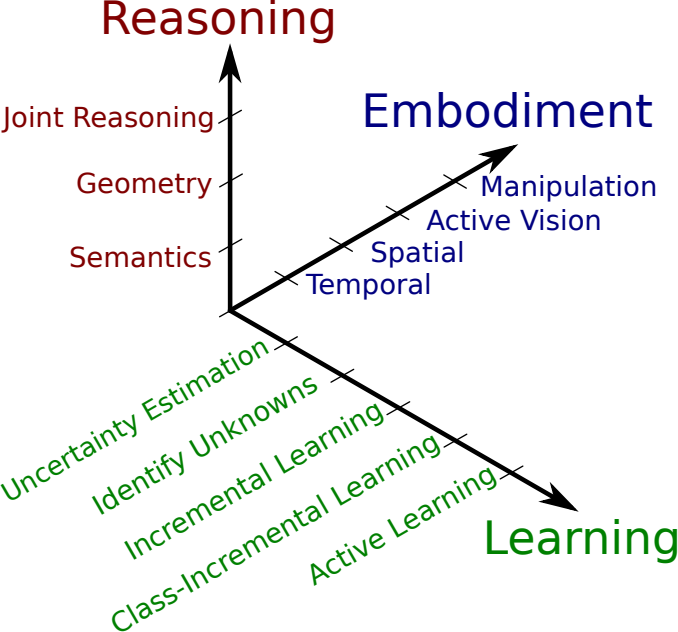
\includegraphics[width=0.75\linewidth]{images/rvchallenges.png}
 	\caption{Current challenges for Deep Learning in Robotic Vision. The authors categorize these challenges into three conceptually orthogonal axes:
 		learning, embodiment, and reasoning. The learning axis is of interest for this thesis. Image from \cite{surveydeeplimits}.}
 \end{figure}
 
 The authors also survey the most most important learning challenges for a (deep) learning machine in a Robotic Vision context. The first is \textit{uncertainty estimation}. An autonomous agent has to estimate the uncertainty of its deep learning modules, considering them in the same way as other sensors. This is not trivial because deep entities return scores that are not calibrated probabilities, so their outputs are not usable in a Bayesian sensor fusion framework, as commonly done in robotics to improve robustness. In Deep Learning, it is assumed that a model operates in \textit{close-set} condition,  i.e., the classes encountered during deployment are known and exactly the same as during training. However, an autonomous agent operates in real-world environments that are uncontrolled and extremely different from each other. In this context, a robot will encounter instances of classes, scenarios, textures, or environmental conditions that were not covered by the training data. On this \textit{open-set} conditions, it is crucial to identify the unknowns, not recognizing them as known classes. Other important challenges for robotics applications using Deep Learning are \textit{incremental learning} and \textit{class-incremental learning}. The characteristics and appearance of objects may change a lot in the deployment scenario compared with the training phase. In addition, real environments often include new objects' categories, not included in the training data. To address this limitation, a Robotic Vision system should be able to learn from new training samples of known and unknown classes collected during deployment. Current techniques for incremental learning imply supervision, in the sense that a human operator has to select and annotate the new data to incorporate in the deep model. \textit{Active learning} is the challenge to overcome this limitation. To minimize user interaction, a robot should be able to select autonomously the best samples to increment the training data and specialize its deep models. In \cite{surveydeeplimits}, \citeauthor{surveydeeplimits} also pose attention on datasets and metrics used to train and evaluate end-to-end modules. As mentioned before, a (deep) model used by an autonomous agent operates in \textit{open-set} conditions when only a small and incomplete knowledge of the real world has been used during training. Following this intuition, the authors argue that the most known and challenging datasets used in Computer Vision (e.g. COCO \cite{coco} or Pascal VOC \cite{pascal}) are not able to model the \textit{open-set} conditions in which a Robotic Vision model operates. This is because they offer a huge amount of data related only to specific object categories, making them unable to represent unknown object classes. Also the metrics (e.g. average accuracy, area under the curve, precision, recall) are not able to measure the uncertainty. These measures compute the best summary statistic over a canned dataset, so they do not generalize well to the entire problem. These metrics indicate that a dataset has been solved, but it does not necessarily mean that the problem itself has been solved.  
 
 
 \section{The Role of Simulation for Robotics}
 \label{sec:importanceofsimulation}
 As argued by \citeauthor{surveydeeplimits} in \cite{surveydeeplimits}, there is a lack of vision datasets for robotic applications, so data collection is a crucial phase to exploit a Robotic Vision task. Modern deep learning models are extremely data hungry: they need a large amount of data to converge and the examples must be as heterogeneous as possible. Besides the size, a well-formed dataset usable in Robotic Vision applications should be able to well generalize the problem it represents. The images should be captured from different positions, heights, and illumination conditions to emulate the freedom of movement that characterizes an autonomous robot. In addition, the examples should be collected from a large numbers of scenes and building types, considering indoor environments with different designs, furniture styles, and structural features. A single object radically changes its appearance based on the context to which it belongs. To collect a dataset from the real world is extremely time expensive and costly. This is because the high number of robot runs to perform, the large amount of environment to consider, and the physical configuration of the active agent employed. To cope with these limitations, simulations are widely used for this purpose. 
 
 Gibson Environment, presented in \cite{gibson}, is a real-world perception framework that can be used to acquire the necessary examples for developing robotic visual perception models. Gibson virtualizes scanned real spaces, rather than using artificially designed ones. Through Gibson, an arbitrary agent (e.g. a small robot as a Turtlebot \cite{turtlebot2, turtlebot3}, a humanoid, or a car) can be simulated respecting its physical constraints, as well as those of the real world. Gibson provides a stream of visual observations from arbitrary viewpoints as if the agent had an on-board camera. The observations include RGB images, depth data, and semantic information, to exploit the complexity of real-world environments. The main goal of Gibson is to bridge the gap between frames that come from its rendering engine and those captured directly from the real world. This is done by using a neural network rendering approach, that combines two functions: the first to make rendered frames look like the real ones, while the latter makes real images look like renderings. These two functions are trained to produce equal outputs, unifying the two domains. Gibson’s underlying database of spaces includes 572 full buildings composed of 1447 floors. Furthermore, the authors also integrate the datasets of Stanford 2D-3D \cite{stanford2d3d} and Matterport3D \cite{matterport} in Gibson for easy use. Both of these are large-scale indoor spaces dataset, that provides semantic annotations to obtain ground truth in vision tasks. In particular, the first offers 6 scanned areas from 3 real buildings of mainly educational and office use, while the former contains 90 scenes scanned from real indoor environments of any kind.
 
  \begin{figure}[h!]
 	\centering
 	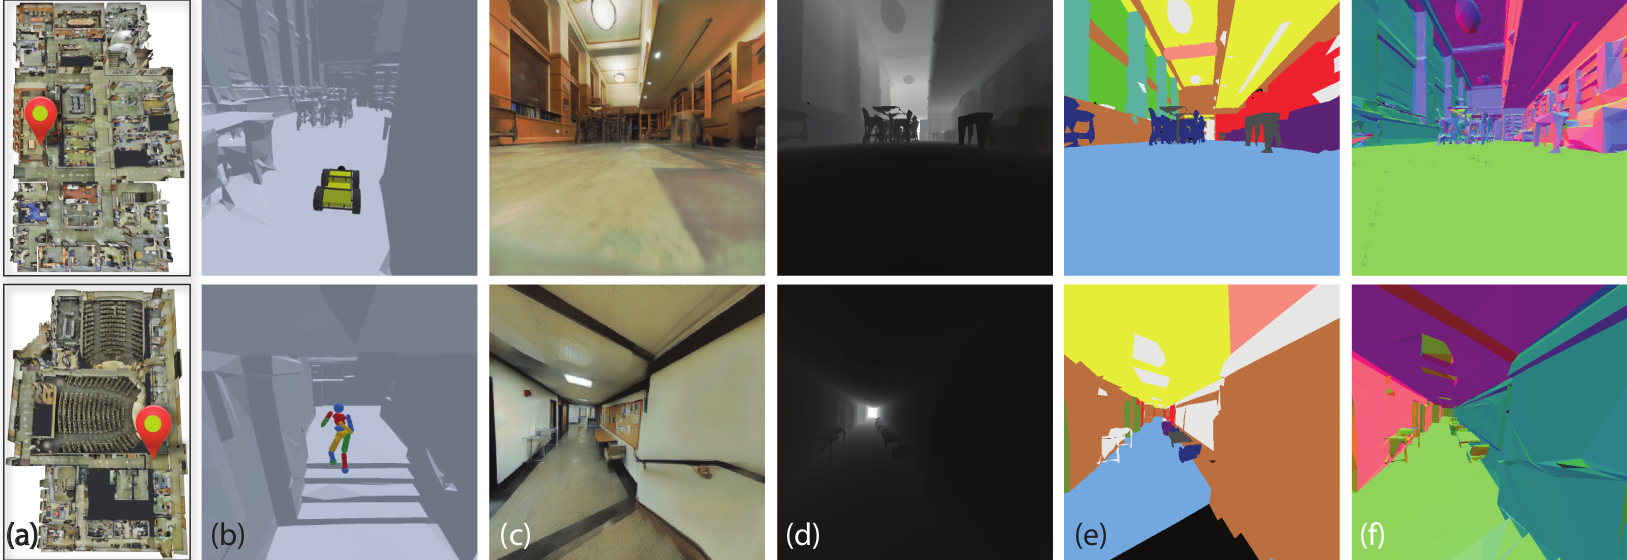
\includegraphics[width=0.99\linewidth]{images/gibson.png}
 	\caption{Two agents in Gibson Environment for real-world perception. The agent is active, embodied, and subject to constraints of physics and space
 		(a, b). It receives a constant stream of visual observations as if it had an on-board camera (c). It can also receive additional modalities, e.g. depth, semantic
 		labels, or normals (d, e, f). Image from \cite{gibson}.}
 \end{figure}
 
 Habitat is a platform for research in embodied artificial intelligence (AI) presented in \cite{habitat}. Habitat framework is composed by two modules: \textit{Habitat-Sim} and \textit{Habitat-API}. \textit{Habitat-Sim} is a flexible, high-performance 3D
 simulator with configurable agents, multiple sensors, and
 generic 3D dataset handling (with built-in support for Matterport3D \cite{matterport}, and Gibson \cite{gibson}). It is extremely fast when rendering a scene from Matterport3D, achieving thousand frames per second in a single thread and over 10,000 fps on a single GPU. \textit{Habitat-API} is a modular high-level library for end-to-end development of embodied AI algorithms concerning navigation, instruction following,
 and question answering.   
 
 In \cite{igibson}, \citeauthor{igibson} propose the Gibson Environment's evolution, called iGibson. This framework aims to unify several aspects of robot simulation, such as physics simulation for object interaction, high-quality simulated sensors data (RGB, depth, segmentation, LiDAR, and so on), integration with reinforcement learning frameworks, and realistic indoor scenes that reflect the objects' distribution of real indoor environments. This robotic simulator contains 15 fully interactive and visually realistic scenes with a total of 108 rooms. These scenes are generated  by annotating 3D reconstructions of real-world scans. The static meshes are then semantically annotated to obtain the ground truth segmentation of the various objects that populate a real scene. Then, these static environment models are converted into fully interactive scenes. This allows embodied active agents to engage in physical manipulation of articulated objects, changing the input sensor signals and the environment state. Furthermore, iGibson offers domain randomization procedures for materials (both visual appearances and dynamics properties) and object shapes applied to the object models in a scene. This facilitates the training of more robust end-to-end modules and improves their generalization properties in unseen scenes. In addition to the 15 interactive scenes, the authors support importing other datasets, such as CubiCasa5k \cite{cubicasa} and 3D-Front \cite{3dfront}. The first is a semi-automatically generated dataset of five thousand annotated floor plans of real-world homes in Finland, while the former is a large dataset of layouts designed by artists and interior designers. Both of them are converted from static scenes to fully interactive environments keeping their original structure. 
 

 